\documentclass[border=2mm]{standalone}
\usepackage{tikz}
\begin{document}
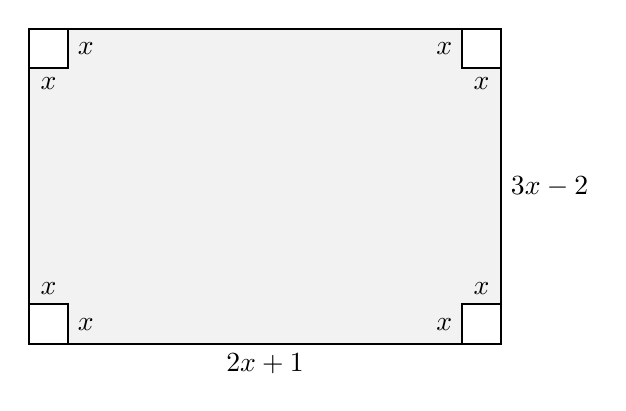
\begin{tikzpicture}
   %\draw[step=1cm,gray,very thin] (-1,-1) grid (7,5);

   \filldraw[gray!10!white, thick, draw=black] (0,0) rectangle (6,4);
   \node at (3,-0.25) {$2x+1$};
   \node [right] at (6,2) {$3x-2$};

   \filldraw[white, thick, draw=black] (0,0) rectangle (.5,.5);
   \filldraw[white, thick, draw=black] (0,3.5) rectangle (0.5,4);
   \filldraw[white, thick, draw=black] (5.5,0) rectangle (6,0.5);
   \filldraw[white, thick, draw=black] (5.5,3.5) rectangle (6,4);

   \node [right] at (0.5,0.25) {$x$};
   \node [above] at (0.25,0.5) {$x$};
   
   \node [left] at (5.5,0.25) {$x$};
   \node [above] at (5.75,0.5) {$x$};

   \node [right] at (0.5,3.75) {$x$};
   \node [below] at (0.25,3.5) {$x$};

   \node [left] at (5.5,3.75) {$x$};
   \node [below] at (5.75,3.5) {$x$};

\end{tikzpicture}
\end{document}
